% ================================== HEADER ====================================
\documentclass{article}           % Sets style/look of many things.
% \documentclass{report}          % part, chapters, front page etc.
\usepackage{exsheets}
\usepackage[utf8]{inputenc}       % Encoding of input files UTF-8
\usepackage[T1]{fontenc}
\usepackage[scaled]{beramono}     % Font
\usepackage{color}                % Color text
\usepackage{titlesec}             % Select alternative section titles
\usepackage{fancyvrb}
\usepackage{verbatim}             % Comment environment
\usepackage{listings}             % Format and render text/code etc.
\usepackage{float}                % Control of floating environment/figure
\usepackage{graphicx,  subfigure} % Better figures, graphics, units etc.
\usepackage{multicol}             % Multiple columns
\usepackage{amsmath}              % Math: Equation, split, align etc.
\usepackage{siunitx}              % SI units
\usepackage{mathtools}            % Different math tools to use with amsmath
\usepackage{amssymb}              % Math symbols
\usepackage[
    colorlinks,
    citecolor=black,              % I like links with standard black color
    filecolor=black,
    linkcolor=black,
    urlcolor=black
]{hyperref}                       % Links in TOC etc.
\usepackage[all]{hypcap}          % Better links to floating environment

\usepackage{tabto}
\newcommand\marginsymbol[1][0pt]{%
  \tabto*{0cm}\makebox[\dimexpr-1cm-#1\relax][r]{$\mathbb{P}$}\tabto*{\TabPrevPos}}

\renewcommand{\thesubsection}{\thesection.\alph{subsection}}
\title{\vspace{-2cm}EMNE Exercise Solutions - Week 1}
\input{../authors1_assignment.tex}
\date{\today}

% Removing paragraph indents is sometimes useful:
\setlength\parindent{0pt}

% Make margins smaller to fit more figures, tables etc on page: (optional)
\addtolength{\oddsidemargin}{-1.0in}
\addtolength{\evensidemargin}{-1.0in}
\addtolength{\textwidth}{2.0in}
\addtolength{\topmargin}{-0.8in}
\addtolength{\textheight}{1.6in}
% ==============================================================================

% ================================= DOCUMENT ===================================
\begin{document}
    \renewcommand\marginsymbol[1][0pt]{%
  \tabto*{0cm}\makebox[-1cm][c]{$\mathbb{P}$}\tabto*{\TabPrevPos}}

\maketitle
\(\mathbb{P}\) marks the programming exercises, using ``Program language'' to run the programs


\section{Simple search algorithms}

Given task

\subsection{Derivative}
Question 

\textit{Answer:}

\subsection{Plotting \marginsymbol}
Given task for plotting:

\emph{Plot:}
\begin{figure}[H]
\begin{center}
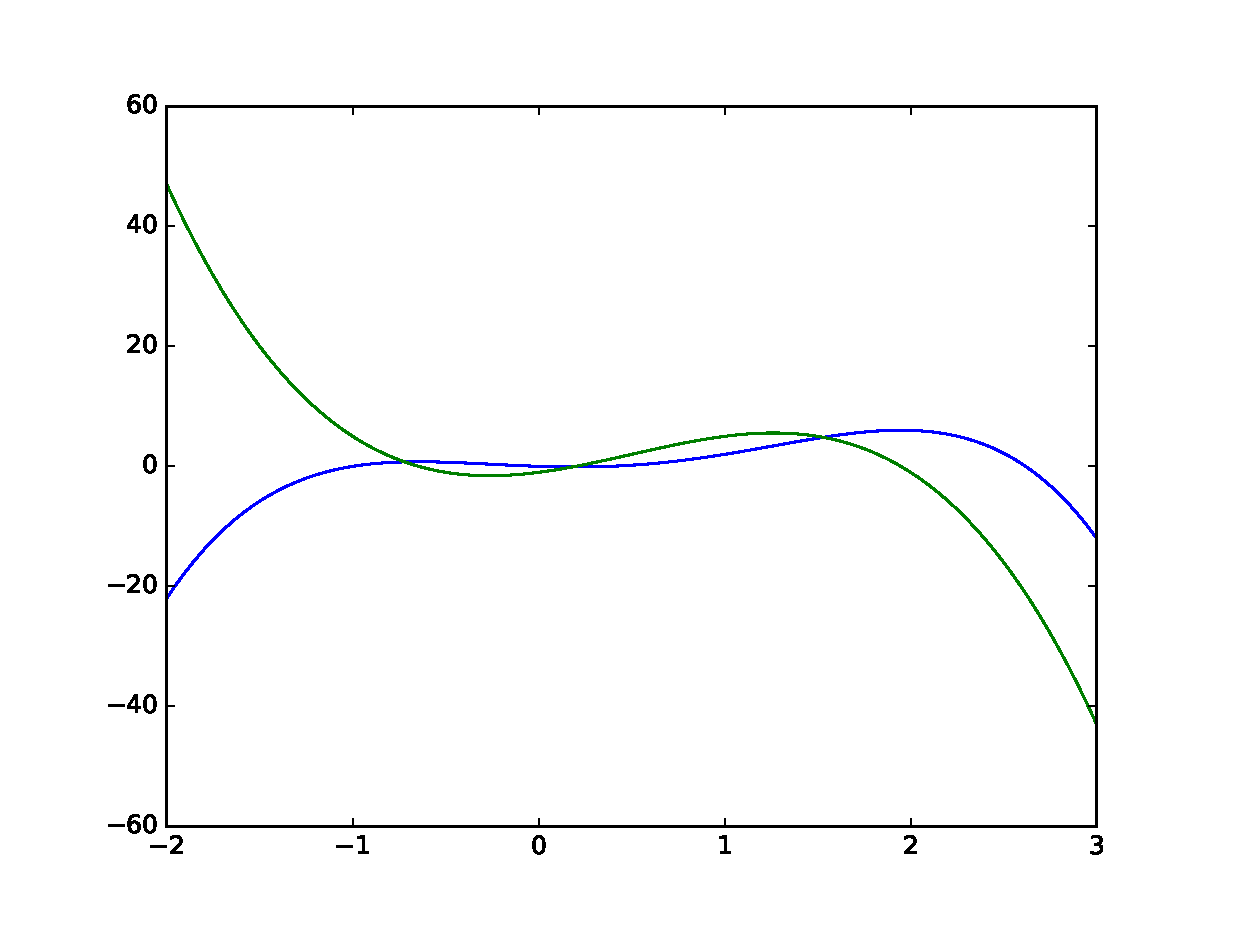
\includegraphics[width=0.6\textwidth]{eps/w1e1b.eps}
\caption{\(f(x)\) and it's derivative.}
\label{fig:w1e1b}
\end{center}
\end{figure}

\emph{Source code (Python 3):}
Source code if needed

\subsection{Gradient Ascent \marginsymbol}
\label{subsec:grada}
Given question

\textit{Answer:}

answer with list, plot and code:

Both starting position and step size affects where the algorithm ends:
\begin{itemize}
    \item Starting Position
    \begin{itemize}
        \item \emph{Left side:} Should converge on left maximum
        \item \emph{Center:} Stops immediately, gradient is zero.
        \item \emph{Right side:} Should converge on right maximum
    \end{itemize}
    \item Step Size
    \begin{itemize}
        \item \emph{Too low:} Converges slowly (poor performance)
        \item \emph{Too high:} Overshoot, bounce over solutions. Doesn't converge, might not terminate.
    \end{itemize}
\end{itemize}

\emph{Plot:}
\begin{figure}[H]
\begin{center}
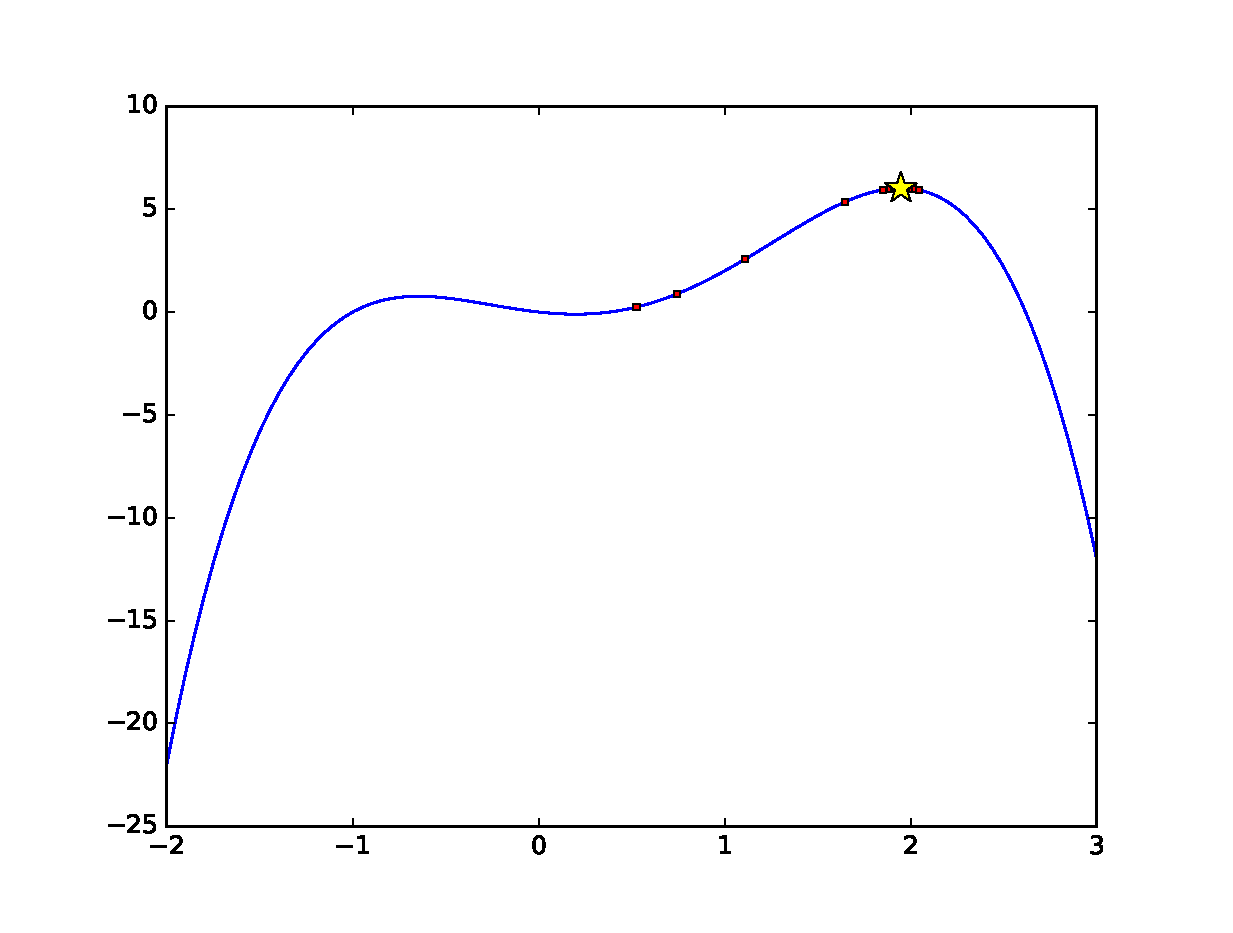
\includegraphics[width=0.6\textwidth]{eps/w1e1c.eps}
\caption{Result of gradient ascent}
\label{fig:w1e1c}
\end{center}
\end{figure}

\emph{Source code (Python 3):}

\end{document}
% ==============================================================================
